\section{データの形を見る}

  \subsection{問い}

    前章では, データを統計量に要約した.
    たくさんの数字を一つにまとめれば扱いやすく, どんなデータなのか, おぼろげに見えてくるのだった.
    ただその一方で, まとめる過程で多くの情報が失われてしまうことも, すでに述べたとおりだ.

    この失われる情報の中には, データ全体がどんな姿をしているか, という大事なものが含まれてしまっている.
    全体の情報も見ることができるとデータの傾向を確認できたりしそうだが, 平均や標準偏差をいくら並べても, それは戻ってこない.

    なんとか, データをそのまま目で見られないだろうか.
    一つひとつの値を残したまま, 全体を一度に捉えたい.
    そこで, 数字の羅列を図にしてみる.

  \subsection{素朴な方法と限界}

    このデータを図にして分かりやすく示してみよう, というとグラフを描くのがよさそうだ. 
    棒グラフや円グラフならニュースでよく見るし, それくらいできるはずだが, 実際にやってみようとすると意外とうまくいかない.
    たとえば映画の視聴回数を棒グラフにするなら, 一本ずつ棒の高さにして横に並べればよい. 
    ところが, 映画を並べる順番に決まりはないから, どう並べ替えても高さのまちまちな棒が立ち並ぶだけで, 全体がどうなっているのかは見えてこない.
    単純に見える数字をグラフにするだけではうまくいかないみたいだ.
    そこで, 今度は近い視聴回数どうしをまとめてみる.
    いくつかの区間に分けて, 区間ごとに何本入るかを数え, その数を棒の高さにする.
    すると, 映画がどのあたりに多く集まっているのか, 全体のかたよりが見えてくる.

    つまり, データを見ればおのずと可視化の仕方が決まる, というものではないし, もっといえば「こういうデータにはこう」と機械的に決められるものでもない. 
    「全体の姿」といっても, どのデータにもただ一つに定まる正解があるわけではないのだ. 
    そうすると, 問題はデータの可視化を, そのデータの全体的な情報として意味を持つようにしなければならないということのようだ.

  \subsection{理論の最小核}

    手がかりは, 先ほどの図にある.
    一本ずつの棒を眺めても何も見えなかったのに, 区間にまとめて数え直したら, 映画の集まり方のかたよりが見えた.
    このとき見えたのは, どの映画が何回見られたか, ではない.
    視聴回数という値がどのあたりに多く, そこからどんなふうに散らばっているのか, という全体の形だ.
    一本ごとの区別を手放した代わりに, 全体の形が見えた.
    この, 値がどこに多くどこに少ないかという散らばりの形を, データの\textbf{分布}と呼ぶ.

    形が見えると, 前章の統計量だけでは区別のつかなかったことに気づける.
    たとえば, 平均も標準偏差もほとんど同じなのに, 山が一つのデータと二つのデータ, ということがありうる.
    数字が同じでも, 形は別物だ.
    そして, 山が二つ見えたなら, 性質の違う映画が混ざっているのではないか, という次の疑問が生まれる.
    図を描いて気づき, 気づいたことを確かめるために, 次の図を描く.
    可視化はこの往復で進み, 往復のたびに仮説が育っていく.

    一つの集まりの形を見るだけでなく, データをグループに分けて形を並べたり, 二つの量を一枚の図に載せたりして, 見比べることもできる.
    並べてみると, 一つの形を眺めているだけでは見えない違いや関係が目に入ってくる.

    では, どの図を描けばいいのだろう.
    データを眺めてもおのずとは決まらないことは, 棒グラフで確かめたとおりだ.
    決めるのは, データではなく, 自分が何を知りたいかのほうだ.
    一つの量の散らばりの形を見たいのか, グループごとの違いを比べたいのか, 二つの量の関係を探りたいのか.
    知りたいことが定まってはじめて, それを確かめるのに向いた図がしぼられてくる.

    もっとも, 何を知りたいのかがまだ定まらないこともある.
    手に入れたばかりで, どんなデータなのか見当もつかないようなときだ.
    こういうときは, データの様子をつかむこと自体が目的だから, 一つの図に頼らず, いくつもの図を試すことになる.
    描いてみると思いがけないかたよりや特徴に気づき, 確かめたいことが新しく生まれる.
    その確かめのために, また別の図を描く.

    \begin{mybox}{可視化の要点}
      図にすると, データを値の散らばりの形, つまり分布として見ることができる. どの図を描くかは, 何を知りたいかで決まる.
    \end{mybox}


  \subsection{手法}

    知りたいことの型に合わせて, この章では\textbf{ヒストグラム}, \textbf{箱ひげ図}, \textbf{散布図}の三つを使う.
    一つの量がどう散らばっているかを見たいならヒストグラム, いくつかのグループを並べて比べたいなら箱ひげ図, 二つの量の関係を見たいなら散布図だ.
    図の種類はほかにも数多くあるが, よく出てくる目的の大半は, この三つで足りる.

    \subsubsection*{ヒストグラム}

      一つ目の図は, じつはもう描いている.
      視聴回数の範囲をいくつかの区間に分け, 各区間に入る映画の本数を数えて, その本数を棒の高さにした, あの図だ.
      この図をヒストグラムと呼び, 区切ってできた一つひとつの区間を\textbf{階級}, 各階級に入る本数を\textbf{度数}と呼ぶ.
      見た目は棒グラフに似ているが, 表しているものは異なる.
      棒グラフは, ジャンルや原作の有無のように, 種類で分かれた項目を棒の高さで比べる.
      ヒストグラムが扱うのは, 視聴回数のように連続して変わる一つの量で, 棒の高さは, その区間に入るデータの多さを表す.

      %% 図プレースホルダー（ヒストグラム）: ファイル名・キャプション・ラベル・配置は仮
      \begin{figure}[htbp]
        \centering
        \includegraphics[width=\linewidth]{../figures/output/histogram.pdf}
        \caption{視聴回数のヒストグラム}
        \label{fig:histogram}
      \end{figure}

      棒の高低は, 視聴回数がどのあたりに多く, どのあたりに少ないかを表している.
      山が一つか, 離れたところにもう一つ山があるか.
      左右のどちらかに長い裾を引いているか.
      多くの映画が集まる範囲から離れたところに少数の映画がないか.
      平均や標準偏差だけでは見えにくかった散らばり方が, 分布の形として見えてくる.

      ただし, 階級の幅をどう取るかで, 同じデータでも図の印象は変わってしまう.
      細かく区切れば小さな凹凸まで見えるが, たまたまのばらつきまで意味のある山に見えてしまう.
      粗く区切れば形はなめらかになるが, 本来は二つあった山が一つにつぶれて見えることもある.

      そのため, 一枚の図だけでは判断できない.
      階級の幅を変えて何枚か描くと, 幅を変えても残る特徴と, ある幅でしか現れない特徴とに分けて考えられる.
      山の位置や裾の向きが大きく変わらなければ, 比較的安定した特徴と考えてよいだろう.
      反対に, 細かな凹凸が特定の幅でしか現れないなら, 区切り方によって生じた見かけだけの特徴かもしれない.

    \subsubsection*{箱ひげ図}

      ジャンルごとの違いを比べたいとき, ジャンルの数だけヒストグラムを描いて並べる手もあるが, 枚数が増えると見比べるのは難しくなる.
      そこで, 前章の要約を思い出す.
      中央値と四分位数を見れば, データの中心と散らばりのおおよそは押さえられるのだった.
      箱ひげ図は, この要約をひとまとまりの図形に描いたものだ.
      箱の中央の線が中央値を, 箱の下端と上端が第1四分位数と第3四分位数を表す.
      箱の高さは四分位範囲であり, データの中央付近の半分がどれくらい広がっているかを示す.
      箱から四分位範囲の1.5倍より外側に離れた値は, 外れ値として点で示すことが多い.
      ひげの両端は, 外れ値を除いたデータのうち, いちばん小さい値といちばん大きい値を表す.

      %% 図プレースホルダー（箱ひげ図）: ファイル名・キャプション・ラベル・配置は仮
      \begin{figure}[htbp]
        \centering
        \includegraphics[width=\linewidth]{../figures/output/boxplot.pdf}
        \caption{ジャンル別の視聴回数の箱ひげ図}
        \label{fig:boxplot}
      \end{figure}

      要約が一つの図形に収まっているから, 群の数が増えても, 横に並べるだけで済む.
      ジャンル別に並べると, 中央値の高低も散らばりの大きさも, 箱の位置と高さの違いとして一度に見比べられる.
      どの群に飛び抜けた値があるかも, 点の出方で分かる.

      ただし, 中央値や四分位数への要約を経ているぶん, 分布の形そのものは箱ひげ図に残らない.
      山が二つあるような分布でも, 箱とひげの見た目は山が一つの場合とほとんど変わらないことがある.
      形まで確かめたい群には, ヒストグラムを併せて描いて補う.

    \subsubsection*{散布図}

      二つの量の関係を見たいときは, 映画の一本一本を点にして打つ.
      横軸に製作費, 縦軸に視聴回数をとると, 一本の映画は, その製作費と視聴回数が指し示す位置の1点になる.
      こうして全部の映画を点として打った図を散布図と呼ぶ.
      二つの量の関係は, 点の散らばり方に現れる.

      %% 図プレースホルダー（散布図）: ファイル名・キャプション・ラベル・配置は仮
      \begin{figure}[htbp]
        \centering
        \includegraphics[width=\linewidth]{../figures/output/scatter.pdf}
        \caption{製作費と視聴回数の散布図}
        \label{fig:scatter}
      \end{figure}

      二つの量のあいだに, 一方が大きくなるともう一方も大きく（あるいは小さく）なる傾向が見られるとき, 両者には\textbf{相関関係}があるという.
      点の並びが右肩上がりなら, 一方が大きいときにもう一方も大きい. その関係を\textbf{正の相関}と呼ぶ.
      右肩下がりなら, 一方が大きいときもう一方は小さい. その関係が\textbf{負の相関}である.
      点が直線の近くにまとまっているほど相関は強く, 広くばらけて向きがはっきりしないほど, 直線的な相関は弱い.

      関係の方向と強さのほかに, 直線で近似できそうか, 曲線的な関係に見えるか, 飛び抜けた点がないか, いくつかの集まりに分かれていないか, といったことも目で読み取れる.

      散布図には大事な留保がある.
      二つの量が一緒に動いていることは見えても, 一方がもう一方を引き起こしているのか, 別の要因が両方に関係しているだけなのかは, 散布図からは判別できない.
      相関の有無と因果の有無は別物だ.
      その境目をどう扱うかは, 後の章で改めて取り上げる.

  \subsection{実践}

    前章で扱った80本の標本データを使って, 3枚の図を実際に描いてみる.
    視聴回数の散らばりをヒストグラムで, ジャンル別の視聴回数を箱ひげ図で, 製作費と視聴回数の関係を散布図で, それぞれ確かめる.

    \subsubsection*{1枚目: 視聴回数のヒストグラム}

      \begin{figure}[htbp]
        \centering
        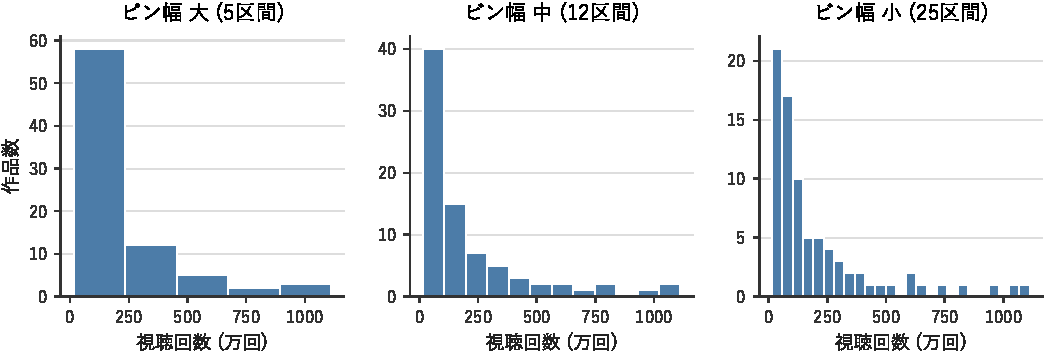
\includegraphics[width=\linewidth]{../figures/output/ch03_histogram.pdf}
        \caption{80本の視聴回数のヒストグラム. 階級の幅を3通りに変えて表示. 縦軸の目盛りは図ごとに異なる.}
        \label{fig:ch03_histogram}
      \end{figure}

      まず, 視聴回数の散らばり方を見るために, ヒストグラムを描く.
      階級の幅を3通り (大・中・小) に変えた図を並べ, 幅を変えても変わらない特徴を確かめる.
      なお, 縦軸 (映画の本数) の目盛りは図ごとに別々なので, 図どうしで棒の高さを直接比べることはできない. 比べるのは分布の形だけだ.

      どの幅で描いても, 視聴回数の少ない側に山があり, 多い側に長く裾を引いている.
      視聴回数の少ない映画が大半で, 右端には視聴回数が桁違いに大きい映画が少数ある.

      前章では, 視聴回数の平均が $209.4$ 万回, 中央値が $107.1$ 万回で, 平均が中央値の約2倍まで膨らんでいた.
      平均をここまで押し上げる映画が, 視聴回数の多い側にあるはずだと推測はできたが, 数値だけでは分布の形までは確かめられなかった.
      ヒストグラムを見ると, 右に裾を引いていることが確認できる.

      この右に裾を引く形は, 80本をひとまとめにして見たときの形だ.
      ジャンルごとに分けたとき, どのジャンルにも同じ形が現れるのか, それともジャンルによって様子が違うのかは, 全体のヒストグラム1枚からは分からない.
      次は, ジャンルで分けて視聴回数を見る.

    \subsubsection*{2枚目: ジャンル別視聴回数の箱ひげ図}

      \begin{figure}[htbp]
        \centering
        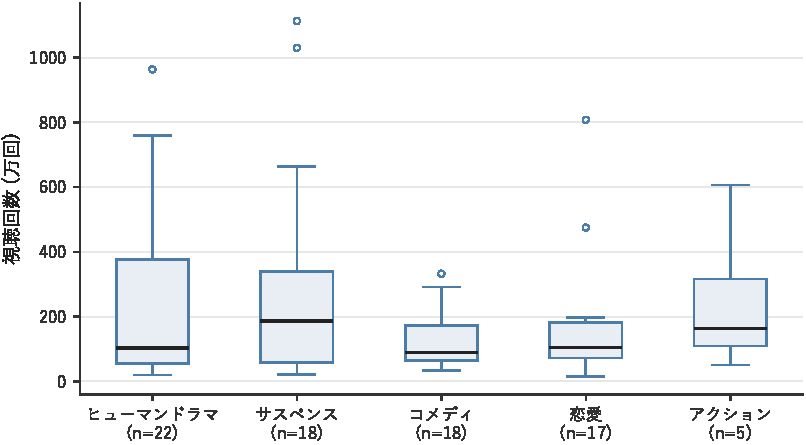
\includegraphics[width=0.85\linewidth]{../figures/output/ch03_boxplot.pdf}
        \caption{ジャンル別（ヒューマンドラマ・サスペンス・コメディ・恋愛・アクション）の視聴回数の箱ひげ図. 各ジャンルの件数を併記.}
        \label{fig:ch03_boxplot}
      \end{figure}

      80本の映画はいくつかのジャンルに分かれている.
      ジャンルごとの視聴回数を比べるために, 横軸にジャンル, 縦軸に視聴回数をとって箱ひげ図を並べる.

      ジャンルによって箱の位置（中央値）が違う.
      箱の高さ（四分位範囲）もジャンルごとに違っていて, 中央値の近くにまとまっているジャンルもあれば, 縦に大きく広がっているジャンルもある.
      ひげの外側にある点（外れ値）の出方も, ジャンルによって違う.
      ジャンルによって, 視聴回数の典型値や散らばりに違いがありそうだ.

      ただし, 同じジャンルの中に, よく見られた映画とあまり見られなかった映画がはっきり分かれて混じっていたとしても, 箱ひげ図の上では見分けがつかない.
      気になるジャンルがあれば, そのジャンルだけヒストグラムを描いて確かめる.

      ジャンルによって視聴回数の典型値や散らばりが違うなら, 視聴回数と一緒に動いている量がほかにもありそうだ.
      手元のデータでまず思い当たるのは製作費だ.
      製作費と視聴回数の関係を, 散布図で見る.

    \subsubsection*{3枚目: 製作費と視聴回数の散布図}

      \begin{figure}[htbp]
        \centering
        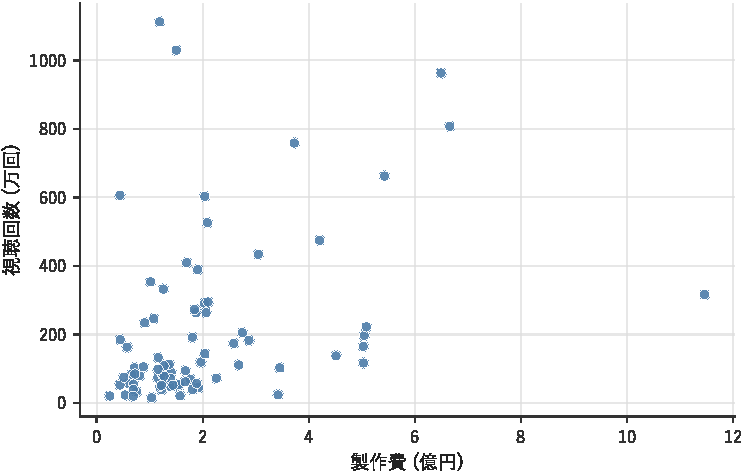
\includegraphics[width=0.8\linewidth]{../figures/output/ch03_scatter.pdf}
        \caption{横軸が製作費 (億円), 縦軸が視聴回数 (万回) の散布図.}
        \label{fig:ch03_scatter}
      \end{figure}

      横軸に製作費, 縦軸に視聴回数をとり, 各映画を点で表す.
      点の並びには, 全体として右肩上がりの傾向が見える.
      製作費が大きい映画ほど, 視聴回数も多い傾向がある.
      ただし関係はきれいな直線ではなく, 製作費が同じくらいの映画どうしでも視聴回数には大きな散らばりがある.

      それでも, この図から言えるのは「正の相関がありそうだ」までで, 「製作費を増やせば視聴回数が増える」とまでは言えない.
      製作費が視聴回数を引き上げているのか, 話題性や宣伝の規模といった別の要因が両方に関係しているだけなのかは, 散布図からは判別できないからだ.

    \subsubsection*{3枚の図から見えたこと}

      視聴回数の全体は右に裾の長い分布で, ジャンルごとに見れば典型値も散らばりも違い, 製作費とのあいだには正の相関がありそうだった.
      1枚目で気づいた形のかたよりが, ジャンルで分ける2枚目につながり, 2枚目で見えた群ごとの違いが, 製作費を横軸にとる3枚目につながった.
      図を描いて気づき, 気づいたことを次の図で確かめる往復を, ここで一巡したことになる.

      この往復で手に入ったのは, 確定した結論ではなく, 次に検証したい仮説だ.
      ジャンル間の差は, 偶然の範囲を超えているのか.
      製作費と視聴回数の関係は, どのくらい強いと言ってよいのか.
      答えるには, 図を眺めるのとは別の方法が必要になる.


  \subsection{結果と次の一手}

    この章では, 統計量だけでは見えにくかったデータの形を, 図にして確かめてきた.
    ヒストグラムで散らばりの形を, 箱ひげ図で群ごとの違いを, 散布図で量どうしの関係を見た.
    見たいことが違えば, 描く図も違う.

    ただし, この章で読み取ったことは, 手元の80本についての結果でしかない.
    別の80本を取り直したら, 視聴回数は同じように右に裾を引くだろうか.
    ジャンルによる差は同じように出るだろうか.
    製作費と視聴回数の関係は同じくらい強いだろうか.
    取り直すたびに同じ結果になるとは限らない.

    取り直したときに結果がどう変わるかが分からないと, 図から読み取ったことが手元の80本にだけ当てはまるのか, それとも背後にある集まりの性質を映しているのかを区別できない.
    次章では, 取り直したときに結果がどれだけばらつくかを見積もる方法を考えていく.
